\cotefile{12}
\scanpage{22}
% archive sheet number: 21
% Several mathematical slots in this typescript were never filled: spacing below preserves them without supplying symbols.
% A long oblique cancellation crosses the Remplaçant paragraph; its exact upper scope is uncertain.
% The pale upper extension is visible between the second and third lines. No verbal text is supplied in the empty formula slots.
\rlap{O}or par raison de platitude $H'_i=\underline{\mathrm{Hom}}\,(\underline{O}_{X'}/J',G'_i)$, donc on peut suppose\unsure{r} (quitte à remplacer les $G_i$ par les $H_i$) que les $G_i$ sont annulés par $J$. \deleted{Remplaçant maintenant $X$ par $\operatorname{Spec}(\underline{O}_X/\underline{J})$, on est ramené au cas où $F$ est un Module fidèle, donc $X$ est irréductible de point générique l'unique point $x\quad\operatorname{Ass}F$. En vertu de théorème de platitude générique, il existe un voisinage ouvert \rlap{U}affine $U$ de $x$ tel que l'anneau de son image inverse $U'$ dans $X'$ soit \uline{libre} sur celui de $U$. Passant \deleted{\unsure{au|en}} à l'interprétation en termes de modules sur ces anneaux, on voit alors aussitôt que \deleted{sur $U'$, l'intersection des} $\quad{}'$ est rulle sur $U'$. Or en vertu de \unsure{\rlap{\S}par|par} \handwritten{3.3.} on a $\operatorname{Ass}F'\quad X'_x\quad U'$, donc $\quad{}'=0$, Supposons maintenant $n\quad 1$, \mbox{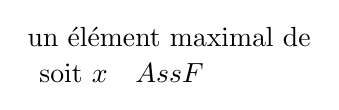
\begin{tikzpicture}[baseline=(base.base),x=1cm,y=1cm]
\node[anchor=west,inner sep=0] (base) at (0,0) {soit $x\quad\operatorname{Ass}F$};
\node[anchor=west,inner sep=0] at (-.15,.45) {\inserted{un élément maximal de}};
\end{tikzpicture}}, d'après ce qui précède, \deleted{il existe un voisinag} si $U$ est un voisinage ouvert de $x$ ne contenant aucun autre \unsure{\rlap{l}élément|Élément|élément} de $\operatorname{Ass}F$, $U'$ son image inverse dans $U$, alors on a $\quad{}'\ U'=0$. En d'autres termes, si $i\colon U\quad X$ est l'imm can, et $v\colon F\quad i\ (F\ U)$ l'homomorphisme canonique, donc le transformé par $\otimes_X X'$ s'identifie à $v'\colon F'\quad \rlap{\(v\)}i'\ (F'\ U')$, \deleted{alors} (réf), alors $\quad{}'$ est une section de $\operatorname{Ker}v'=\operatorname{Ker}v\otimes_X X'$ (re-platitude). Introduisant $F_1=\operatorname{Ker}v$, on peut donc considérer $\quad{}'$ comme une section de $F'_1$, et on est ramené au problème précédent avec $F$ remplacé par $F_1$. Mais $\operatorname{Ass}F_1=\operatorname{Ass}F-x$, et on gagne par hyp de récurrence. (NB au lieu de récurrer sur $\operatorname{card}\operatorname{Ass}$ on peut aussi dans ce dernier argument envisager qu'on a fait une récurrence \deleted{sur} noethérienne sur $\operatorname{supp}F$, ce qui est plutôt plus naturel et dispense de vérifier une formule à la noix sur $\operatorname{Ass}F_1$).}

Bien entendu, prop. \handwritten{3} a) (ii) résulte de là, car on y peut supposer $X$ et $X'$ affines, les $Z_i$ affines (quitte à remplacer chaque $Z_i$ par des ouverts affines le recouvrant), et on applique le critère 1. (iii) en notant que les $u_i\ (\underline{O}_{Z_i})$ sont bien quasi-coh.
